\chapter*{Введение}\label{sec:secIntro}
\addcontentsline{toc}{chapter}{Введение}

Исследование уравнения состояния ядерного вещества --- одна из важнейших проблем современной физики. В обычных условиях ядерная материя существует в виде нейтронов и протонов, связанных друг с другом благодаря сильному взаимодействию. При изменении плотности и температуры изменяется состояние ядерного вещества, возможны фазовые переходы. Теория, описывающая сильные взаимодействия --- квантовая хромодинамика (КХД), еще далека от завершения и нуждается в расширении эмпирической базы. Перед учеными стоит задача определить границы существования различных фаз и описать их свойства. Совокупность теоретических представлений по данному вопросу качественно отображается на фазовой диаграмме, см.~\figref{fig:PhaseDiagram}. Здесь по горизонтальной оси отложен барионный химический потенциал $\mu_{B}$, связанный с плотностью барионов $\rho_{B}$, а по вертикальной --- температура $T$. Область высокой температуры и малой плотности соответствует ранней вселенной, когда нуклоны еще не были сформированы. Область больших плотностей и малых температур реализуется в глубине нейтронных звезд. В земных условиях получение сгустка ядерного вещества с повышенными температурой и плотностью, т.н. файербола (fireball), возможно в столкновениях тяжелых ионов. Актуальные экспериментальные исследования направлены на установление границы между барионной материей, состоящей из адронов, и кварк-глюонной плазмой (КГП), локализацию критической точки и исследование свойств материи в доступных областях фазовой диаграммы~\cite{CBMBook}.
На~\figref{fig:PhaseDiagram2} для материи с нулевой странностью и отношением зарядового числа к барионному $Q/B=0.4$, показаны в координатах ($T$, $\rho_{B}$) условия адронизации (hadronic freeze-out), достижимые в столкновениях тяжелых ионов золота. Теоретическое обоснование приведенной кривой содержится в работе~\cite{Randrup}.
% Источник картинки указан в подписи к картинке
% Собственно именно в том виде, что она вставлена сюда, картинка взята из CBM physics book, page 864

\begin{figure}[H]
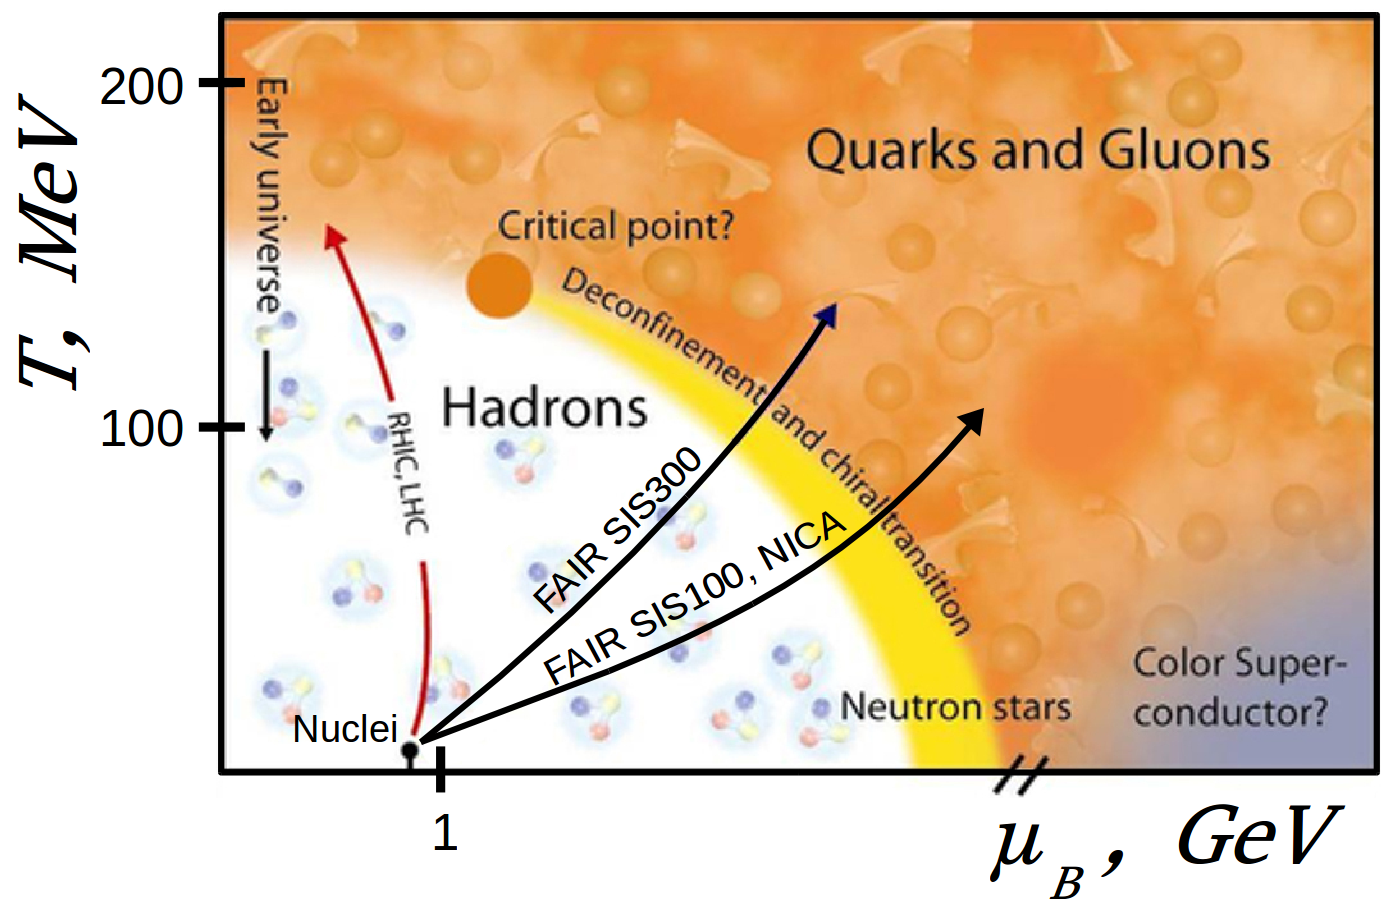
\includegraphics[width=0.8\textwidth]{pictures/QGP_phase_diag_3.png}
\caption{Фазовая диаграмма барионной материи.}
\label{fig:PhaseDiagram}
\end{figure}

\begin{figure}[H]
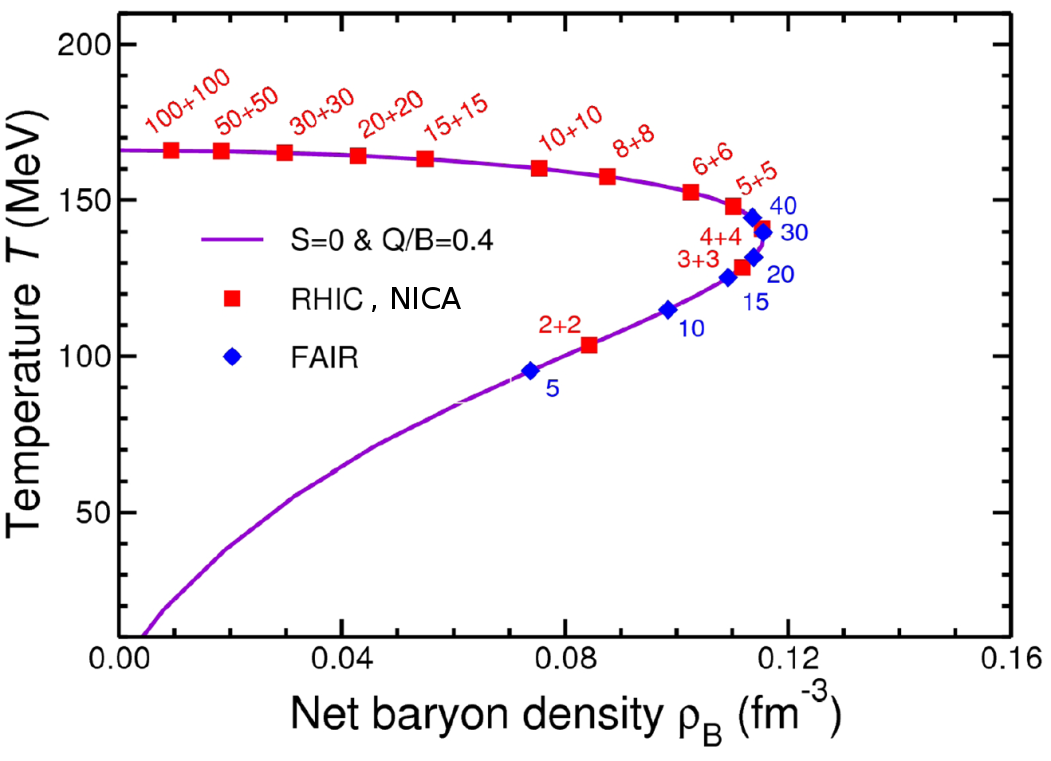
\includegraphics[width=0.8\textwidth]{pictures/Phase_diag.png}
\caption{Термодинамические параметры $T$ и $\rho_{B}$, при которых происходит адронизация при столкновениях ионов золота, по материалам работы~\cite{Randrup}. Синий --- режим с фиксированной мишенью на FAIR, красный --- режим встречных пучков на RHIC и NICA.}
\label{fig:PhaseDiagram2}
\end{figure}

На~\figref{fig:LittleBang} показана схема эволюции файербола, образованного при столкновении двух тяжёлых ионов в лаборатории.
Информация о свойствах ядерной материи в той или иной области фазовой диаграммы может быть извлечена из анализа наблюдаемых, чувствительных к состояниям, в которых находился файербол в момент ``вымораживания'' тех или иных частиц.

\begin{figure}[H]
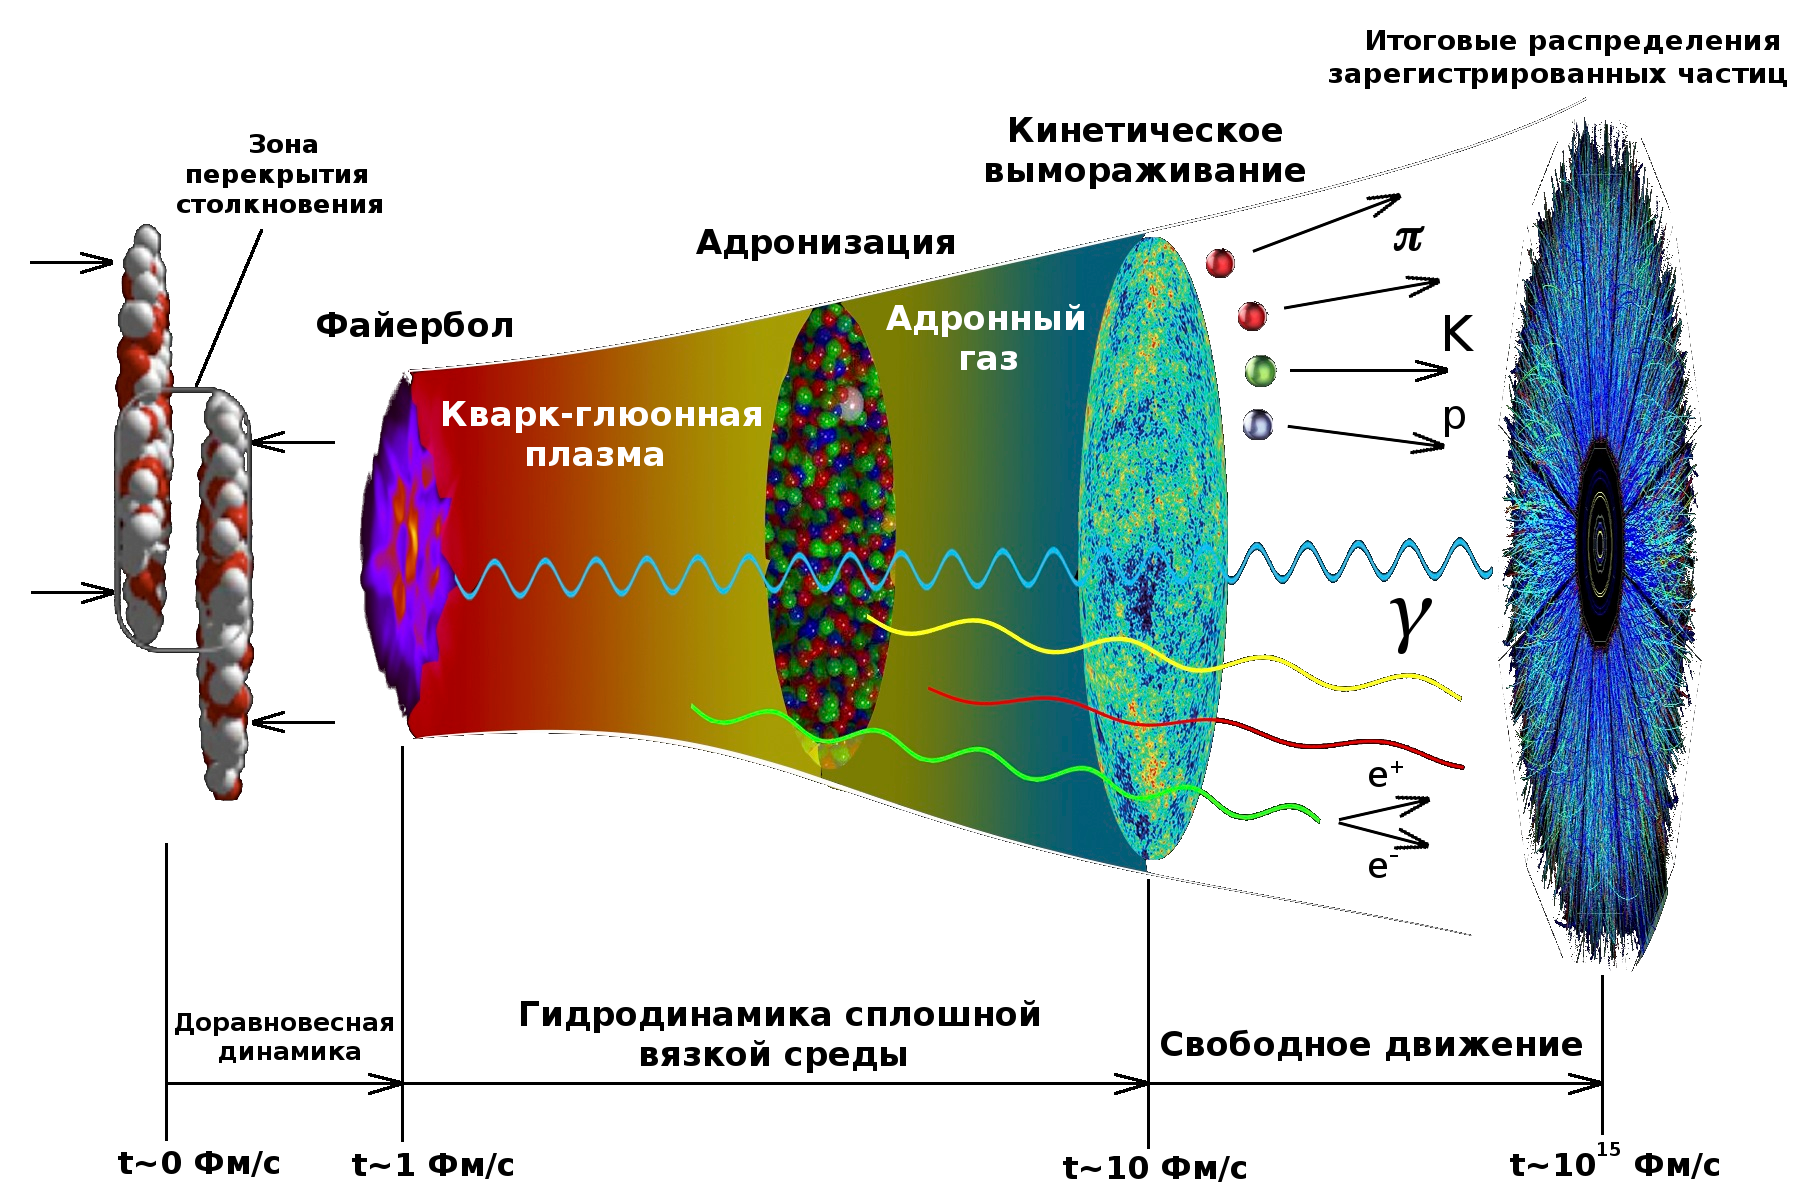
\includegraphics[width=1.0\textwidth]{pictures/little_bang_rus2.png}
\caption{Этапы релятивистского столкновения тяжёлых ионов (courtesy of Paul Sorensen and Chun Shen \todo).}
\label{fig:LittleBang}
\end{figure}
% Paul Sorensen and Chun Shen

Разные наблюдаемые рождаются на разных этапах столкновения, следовательно, их индивидуальные и коллективные параметры несут информацию о разных состояниях вещества, существовавших в разное время после столкновения первичных ионов. Наибольший интерес представляют следующие наблюдаемые.

\begin{itemize}
\item Выходы и спектры адронов, содержащих легкие кварки и рождающихся в больших количествах($\pi^{+}$, $\pi^{-}$, $p$), несущие информацию о таких термодинамических параметрах как давление и температура в момент адронизации.
\item Выходы и спектры странных и очарованных адронов, которые должны быть чувствительны к явлению деконфайнмента.
\item Анизотропия выходов и спектров (elliptic flow \todo) адронов, содержащих $u$, $d$ и $s$ кварки (чему, бишь, нас это учит \todo) 
\item Коррелляции адронов, содержащих легкие и странные кварки, позволяющие исследовать локальные многопартонные взаимодействия.
\item Выходы прямых фотонов и дилептнонные распады легких векторных мезонов ($\rho$, $\omega$, $\phi$) и частиц со скрытым очарованием ($J/\phi$, $\psi'$), несущие информацию о состоянии файербола на ранних стадиях столкновения.
\item Выход странных и очарованных частиц вблизи порога рождения. Эти наблюдаемые несут информацию о коллективных взаимодействиях партонов.
\item Значительные, превышающие статистически ожидаемые, флуктуации от события к событию выходов адронов, содержащих различные ароматы кварков. Такие флуктуации являются индикатором достижения критической точки.
\item Модификация масс адронов, рождающихся и распадающихся в плотной среде, может свидетельствовать о восстановлении киральной симметрии при высоких плотностях.
\item Выходы дважды странных гиперонов, гиперядер, тяжелых мультистранных короткоживущих объектов несут информацию о каскадных процессах, чувствительных к локальным флуктуациям плотности и диффузии странности в плотной среде.
\end{itemize}

% \todo пунктуация
Исследование неравномерности поведения перечисленных наблюдаемых в зависимости от массы и энергии в системе центра масс сталкивающихся ядер, а также от центральности соударений, может позволить обнаружить признаки фазовых переходов.

На~\figref{fig:CBMParticlesYields} показана вероятность рождения различных регистрируемых и восстанавливаемых частиц при центральном столкновении ионов золота с энергией в системе центра масс $\sqrt{s_{NN}}$=\todo~\GeVperNucl{}. Вероятность представлена как произведение полной множественности вторичных частиц на относительную вероятность рождения данной частицы. В правой части рисунка находятся частицы, регистрация которых требует максимальной статистики.

\begin{figure}[H]
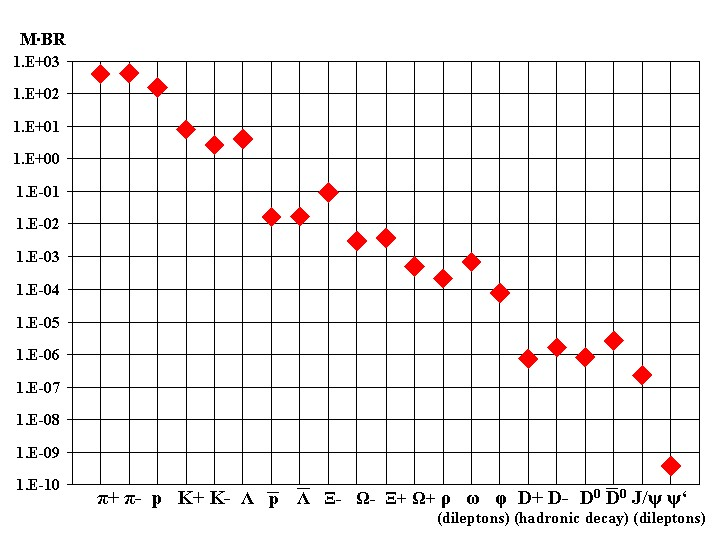
\includegraphics[width=0.8\textwidth]{pictures/CBM_observables.png}
\caption{Основные наблюдаемые CBM~\cite{CBMBook}. По горизонтальной оси --- восстанавливаемая частица, по вертикальной --- произведение множественности на коэффициент ветвления, характеризующее ожидаемую статистику.}
\label{fig:CBMParticlesYields}
\end{figure}

%\todo \textbf{Дать ссылку на источник? Я взял это из CBM Physics Book стр. 866.} Страницу или секцию как-то указать?

% ------------------------------------------------------------------
% ------------------------------------------------------------------
% ------------------------------------------------------------------

Наиболее важные действующие эксперименты в области исследования столкновений тяжелых ионов --- это STAR на ускорителе релятивистских тяжелых ионов (RHIC) в Брукхейвене, США, и ALICE на большом адронном коллайдере (LHC) в ЦЕРН, Женева, Швейцария. Отметим также эксперименты меньшего масштаба NA61 (North Area 61 a.k.a. SHINE --- SPS Heavy Ion and Neutrino Experiment) на синхротроне SPS в ЦЕРН, HADES (High Acceptance DiElectron Spectrometer) --- эксперимент на SIS18 в GSI, BM$@$N (Baryonic Matter at Nuclotron) --- эксперимент на нуклотроне в ЛФВЭ ОИЯИ. Из строящихся экспериментов наиболее важны MPD на ионном коллайдере NICA в Дубне и CBM на ускорительном комплексе FAIR в Дармштадте, Германия. Обсудим некоторые из этих экспериментов подробнее.

\bigskip

% ------------------------------------------------------------------
% ------------------------------------------------------------------
% ------------------------------------------------------------------

% STAR@RHIC

% https://www.bnl.gov/npp/docs/tribble090712/Vigdor_RHIC_overview_rev2.pdf - слайд 7
% 1209546.pdf Abstract

Релятивистский коллайдер тяжёлых ионов (The Relativistic Heavy Ion Collider, RHIC) расположен в Брукхейвенской национальной лаборатории (Brookhaven National Laboratory, BNL), штат Нью-Йорк, США. Первоначально RHIC проектировался для достижения максимально высоких энергий столкновения и предоставлял $\sqrt{s_{NN}}=200$~\GeVperNucl, что соответствует формированию горячей ядерной материи с низкой плотностью. С целью исследования более широкой области фазовой диаграммы, начиная с 2010~г. выполняется скан вниз по энергиям пучка, называемый Beam Energy Scan (BES).

Детекторная установка STAR (Solenoidal Tracker at RHIC) --- это одна из двух ныне действующих установок на RHIC. Основная задача STAR --- исследование формирования и характеристик кварк-глюонной плазмы. В 2011 была завершена первая фаза программы скана со встречными пучками золота с энергий от 7.7~\GeVperNucl{} до 39~\GeVperNucl. Учитывая набранные ранее данные, диапазон энергий $\sqrt{s_{NN}}$, измеренных на RHIC составляет 7.7--200~\GeVperNucl. Этот диапазон энергий столкновения соответствует области фазовой диаграммы, в которой ожидается наличие перехода фазового первого рода и критической точки. Вторая фаза BES, запланированая на 2018--2019~гг, нацелена на исследование столкновений ионов золота при энергиях $\sqrt{s_{NN}}$ от~20 до~7~\GeVperNucl{} в режиме встречных пучков и $\sqrt{s_{NN}}$ от~7 до~3.5~\GeVperNucl{} в режиме с фиксированной мишенью (FXT). Эти измерения, несмотря на низкую статистику, позволят измерить выходы и спектры адронов и определить, опираясь на статистическую термальную модель (THERMUS~\cite{}), параметры состояния на границе адронизации.

\bigskip

% ------------------------------------------------------------------
% ------------------------------------------------------------------
% ------------------------------------------------------------------

% ALICE@LHC

Эксперимент ALICE (A Large Ion Collider Experiment), один из четырёх крупных экспериментов на большом адронном коллайдере (Large Hadron Collider, LHC) ЦЕРН, нацелен на изучение столкновений тяжёлых ионов. Рекордная энергия $\sqrt{s_{NN}}=5.5$~\mbox{ТэВ/нуклон} для сталкивающихся пучков ядер свинца позволяет получить ядерную материю с беспрецедентно высокой температурой. Частота взаимодействий достигает порядка 10~кГц. В эксперименте одновременно сохраняются данные с тремя типами триггеров: с минимальным перекрытием ядер, с высокой центральностью и с отбором редких событий заданного типа.

Высокая температура ядерного вещества приводит к следующим особенностям: процессы с высокой передачей энергии идут с высокой вероятностью, что позволяет тестировать модели пертурбативной КХД; появляется возможность регистрировать $Z^{0}$ и $W^{\pm}$ бозоны, рождающиеся в окружении горячей ядерной материи; возрастает относительное время существования КГП, в результате чего расширение файербола определяется в большой степени динамикой партонов, что проявляется в потоках и спектрах испускаемых адронов; большое значение приобретает регистрация прямых фотонов, несущих информацию о термодинамических условиях на ранней горячей фазе столкновения. Среди интересных результатов, полученных к настоящему моменту на ALICE, отметим компенсацию подавления рождения $J/\psi$ в столкновениях с высокой центральностью. Этот эффект может быть связан с большой концентрацией очарованных кварков и антикварков в среде в момент адронизации. Температура адронизации, достигнутая в ALICE оценивается как T$\approx$160~MeV.

\bigskip

% В этом файле содержится дополнительная информация.
%%\section{ALICE@LHC}

Эксперимент ALICE (A Large Ion Collider Experiment), один из четырёх крупных экспериментов на большом адронном коллайдере (Large Hadron Collider, LHC) ЦЕРН, нацелен на изучение столкновений тяжёлых ионов. Рекордная энергия $\sqrt{s_{NN}}=5.5$~\mbox{ТэВ/нуклон} для сталкивающихся пучков ядер свинца позволяет получить ядерную материю с беспрецедентно высокой температурой. Частота взаимодействий достигает порядка 10~кГц. В эксперименте одновременно сохраняются данные с тремя типами триггеров: с минимальным перекрытием ядер, с высокой центральностью и с отбором редких событий заданного типа.

Высокая температура ядерного вещества приводит к следующим особенностям: процессы с высокой передачей энергии идут с высокой вероятностью, что позволяет тестировать модели пертурбативной КХД; появляется возможность регистрировать $Z^{0}$ и $W^{\pm}$ бозоны, рождающиеся в окружении горячей ядерной материи; возрастает относительное время существования КГП, в результате чего расширение фаербола определяется в большой степени динамикой партонов, что проявляется в потоках и спектрах испускаемых адронов; большое значение приобретает регистрация прямых фотонов, несущих информацию о термодинамических условиях на ранней горячей фазе столкновения. Среди интересных результатов, полученных к настоящему моменту на ALICE, отметим компенсацию подавления рождения $J/\psi$ в столкновениях с высокой центральностью. Этот эффект может быть связан с большой концентрацией очарованных кварков и антикварков в среде в момент адронизации. Температура адронизации, достигнутая в ALICE оценивается как T$\approx$160~MeV.

% http://www.slac.stanford.edu/econf/C060717/papers/L010.PDF

%Эксперимент ALICE (A Large Ion Collider Experiment) --- это один из четырёх крупных экспериментов на большом адронном коллайдере (Large Hadron Collider, LHC), который занимается изучением столкновений тяжёлых ионов.

%The rate of Pb--Pb collisions in 2010 and 2011 was well below the ALICE limits and ALICE was able to take data at the highest achievable luminosity, on the order of $10^25$ $s^{-1}$ $cm^{-2}$ in 2010 and $10^{26}$ $s^{-1}$ $cm^{-2}$ in 2011, with the corresponding hadronic $\mu$ being on the order of $10^{-5}$ -- $10^{-4}$ and $10^{-4}$ -- $10^{-3}$, respectively.

%During the 2011 Pb--Pb running period, the interaction rate provided by the LHC reached 3-4 kHz. ALICE ran with the minimum bias, centrality, and rare triggers activated at the same time. In the LHC Run 2 (2015--2017), for which the expected collision rate is O(10) kHz, still low enough to avoid pileup.

%The LHC at CERN will provide colliding Pb ions with an energy of $\sqrt{s_{NN}}=5.5 TeV$.

%It is expected that the LHC can deliver luminosities of $10^{27}$ $cm^{2}$ $s^{-1}$ for Pb--Pb collisions, which results in a minimum-bias interaction rate of 8~kHz. Lighter ions can be delivered with higher luminosities of up to $10^{29}$ $cm^{2}$ $s^{-1}$, corresponding to an interaction rate of several 100~kHz. The machine can deliver p--p luminosities up to $10^{31}$ $cm^{2}$ $s^{-1}$ but because of detector limitations this luminosity is restricted to $10^{30}$ $cm^{2}$ $s^{-1}$ for ALICE.

%--- Hard processes become abundant.
%The abundance of hard processes at the LHC will allow for precision test of perturbative QCD. In addition, the large jet rates at the LHC permit detailed measurements of jet quenching to study the early stages of the collision.

%--- Access to weakly interacting hard probes.
%Direct photons as well as $Z^{0}$ and $W^{\pm}$ bosons produced in hard processes will provide information about nuclear parton distributions at high $Q^{2}$ . Jet tagging with such probes yields a calibrated energy scale for jet quenching studies.

%--- Fireball expansion is dominated by parton dynamics.
%Due to the expected longer lifetime of the QGP, the parton dynamics will dominate over the hadronic contribution to the fireball expansion and the collective features of the event.

%The charged particle multiplicity per colliding nucleon pair measured by ALICE for the most central collisions is double that measured at RHIC, where the collision energy is factor 14 lower, fig.1. This shows that the system created at LHC has much higher energy density and is at least 30\% hotter that at RHIC. Fig. 2 shows the charged particle multiplicity as a function of the number of participants. 

%One of the classic signals expected for a quark-gluon plasma (QGP) is the radiation of ``thermal photons'', with a spectrum reflecting the temperature of the system. With a mean-free path much larger than nuclear scales, these photons leave the reaction zone created in a nucleus–nucleus collision unscathed. So, unlike hadrons, they provide a direct means to examine the early hot phase of the collision. However, thermal photons are produced throughout the entire evolution of the reaction and also after the transition of the QGP to a hot gas of hadrons. In the PbPb collisions at the LHC, thermal photons are expected to be a significant source of photons at low energies (transverse momenta, $p_{T}$, less than around 5~\GeVoverC{}). The experimental challenge in detecting them comes from the huge background of photons from hadron decays, predominantly from the two-photon decays of neutral pions and ? mesons. 

%Direct photons are defined as photons not coming from decays of hadrons, so photons from initial hard parton-scatterings (prompt photons and photons produced in the fragmentation of jets) --- i.e. processes already present in proton-proton collisions --- contribute to the signal. Indeed, for pT greater than around 4~\GeVoverC{}, the measured spectrum agrees with that for photons from initial hard scattering obtained in a next-to-leading-order perturbative QCD calculation. For lower pT, however, the spectrum has an exponential shape and lies significantly above the expectation for hard scattering, as the figure shows. The inverse slope parameter measured by ALICE, $T_{LHC}$ = 304$\pm$51 (stat.+syst.) MeV, is larger than the value observed in gold-gold collisions at $\sqrt{s}$ = 0.2~TeV at Brookhaven’s Relativistic Heavy-Ion Collider (RHIC), $T_{RHIC}$ = 221 $\pm 19$ (stat.) $\pm 19$ (syst.) MeV. In typical hydrodynamic models, this parameter corresponds to an effective temperature averaged over the time evolution of the reaction. The measured values suggest initial temperatures well above the critical temperature of 150--160 MeV (approx. 1.8 $\times$ 1012 K) at which the transition between ordinary hadronic matter and the QGP occurs. The ALICE measurement also indicates that the LHC has produced the hottest piece of matter ever formed in a laboratory. 

%At the LHC, however, extremely interesting developments are expected. In particular, a much higher number of charm-anticharm pairs are produced in the nuclear interaction, thanks to the unprecedented centre-of-mass energies. As a consequence, even a suppression of the $J/\psi$ yield in the hot QGP phase could be more than counter-balanced by a statistical combination of charm-anticharm pairs happening when the system, after expansion and cooling, finally crosses the temperature boundary between the QGP and a hot gas of particles. If the density of heavy quark pairs is large enough, this regeneration process may even lead to an enhancement of the $J/\psi$ yield --- or at least to a much weaker suppression with respect to the experiments at lower energies. The observation of the fate of the $J/\psi$ in nuclear collisions at the LHC constitutes one of the goals of the ALICE experiment and was among its main priorities during the first run of the LHC with lead beams in November/December 2010.

%The results from the first ALICE run are rather striking, when compared with the observations from lower energies. While a similar suppression is observed at LHC energies for peripheral collisions, when moving towards more head-on collisions --- as quantified by the increasing number of nucleons in the lead nuclei participating in the interaction --- the suppression no longer increases. Therefore, despite the higher temperatures attained in the nuclear collisions at the LHC, more $J/\psi$ mesons are detected by the ALICE experiment in Pb--Pb with respect to p--p. Such an effect is likely to be related to a regeneration process occurring at the temperature boundary between the QGP and a hot gas of hadrons (T$\approx$160~MeV).


% ------------------------------------------------------------------
% ------------------------------------------------------------------
% ------------------------------------------------------------------

Описанные выше эксперименты на RHIC и LHC исходно были нацелены на изучение ядерной материи при высоких температурах и относительно малых значениях барионного потенциала. Большой физический интерес представляет и область фазовой диаграммы с высокой барионной плотностью, которая может быть исследована при столкновениях тяжелых ядер с меньшей энергией. Пионерские исследования в этой области делаются на ускорителе RHIC в программе сканирования по энергиям. Недостатком этих исследований является невысокая частота взаимодействий, что позволяет получить доступ к только ограниченному кругу наблюдаемых. Существуют два пути повышения частоты взаимодействий: (1) оптимизация ускорителя встречных пучков под низкие энергии, что позволит минимизировать эмиттанс пучка при большом значении тока и, следовательно, увеличить частоту взаимодействий и (2) работа с фиксированной мишенью. Первый подход реализуется в проекте MPD на ускорителе NICA в Дубне, а второй --- в проекте CBM на FAIR в Дармштадте.

\bigskip

% ------------------------------------------------------------------
% ------------------------------------------------------------------
% ------------------------------------------------------------------

% MPD@NICA

В Объединённом Институте Ядерных Исследований (ОИЯИ) в г.~Дубне идёт строительство коллайдерного комплекса NICA (Nuclotron-based Ion Collider fAciliy) на базе нуклотрона, который предоставит встречные пучки от протонов до ионов золота в диапазоне энергий в системе центра масс $\sqrt{s_{NN}}$ от~4~\GeVperNucl{} до~11~\GeVperNucl{} и со светимостью $1.5 \cdot 10^{26}$ см$^{-2}$ с$^{-1}$ для $^{197}Au$ при $\sqrt{s_{NN}}=4$~\GeVperNucl{} и $10^{27}$ см$^{-2}$ с$^{-1}$ при $\sqrt{s_{NN}}=11$~\GeVperNucl. Параллельно со строительством комплекса NICA идет создание расположенного на нем эксперимента MPD. Этот эксперимент, помимо выходов и спектров адронов ($pi^{+}$, $K^{+}$, $p$, $\rho$, $\omega$, $\phi$, $\Omega$, $D^{0}$, $J/\psi$), позволит измерить флуктуации от события к событию, исследовать анизотропию выходов адронов и осуществить корреляционные измерения при высокой статистике.

\bigskip

% Sorin_SQM2013_Birmingham_25_07_2013.pdf

% ------------------------------------------------------------------
% ------------------------------------------------------------------
% ------------------------------------------------------------------

% CBM@FAIR

Эксперимент с фиксированной мишенью CBM нацелен на исследование ядерной материи с высокой барионной плотностью и низкой температурой с рекордной статистикой. Частота ядерных взаимодействий в этом эксперименте будет достигать $10^7$~с$^{-1}$. При работе на синхротроне SIS100 энергия в системе центра масс будет достигать для золота $\sqrt{s_{NN}}$ \todo и $\sqrt{s_{NN}}$ \todo при работе на SIS300. В центральных столкновениях плотность может превышать нормальную ядерную в 8--10 раз. Благодаря высокой статистике, CBM будет способен исследовать такие наблюдаемые как флуктуации потоков и спектров адронов от события к событию; анизотропия потоков адронов, в т.ч. странных и очарованных; выходы вблизи порога и свойства в среде лёгких векторных мезонов, $J/\psi$, $D$-мезонов с точностью, недоступной в других экспериментах. Все наблюдаемые могут быть измерены при различных массах ядер, значениях энергии столкновения и центральности, которая характеризует величину файербола.

\bigskip

% ------------------------------------------------------------------
% ------------------------------------------------------------------
% ------------------------------------------------------------------

Достижимые результаты во всех рассмотренных экспериментах во многом определятся статистикой, которую они могут собрать за адекватное время, которая, в свою очередь, определяется частотой первичных взаимодействий. Эта частота ограничена сверху двумя факторами --- интенсивностью пучков ускорителя и пропускной способностью детекторной установки. В таблицу~\ref{tabl:Experiments1} сведены такие базовые параметры рассмотренных выше экспериментов, как энергия в центре масс для столкновений конкретных тяжелых ионов и частота взаимодействий. На~\figref{fig:Experiments} более подробно представлены параметры экспериментов, работающих с относительно высокой барионной плотностью.

% \todo В таблице в каждой строке указать Pb+Pb или Au+Au.

\begin{table}[H]
\caption{Показатели экспериментов в области исследования сверхплотной материи.}
\label{tabl:Experiments1}
\begin{tabular}{ | p{0.21\linewidth} | p{0.16\linewidth} | p{0.33\linewidth} | p{0.17\linewidth} | }
\hline
Эксперимент & Тип установки & Диапазон энергий (Au/Pb) & Частота взаимодействий, Гц \\
\hline
\scriptsize{STAR \newline RHIC, BNL, \newline Нью-Йорк, США} & \scriptsize{Встречные пучки} \newline \scriptsize{Фикс. мишень}\footnotemark[1] & $\sqrt{s_{NN}}$=7--200 \GeVperNucl & 1--800 \\
\hline
\scriptsize{NA61/SHINE \newline SPS, CERN, \newline Женева, Швейцария} & \scriptsize{Фикс. мишень} & $E_{kin}$=20--160 \GeVperNucl \newline $\sqrt{s_{NN}}$=6.4--17.4 \GeVperNucl & 80 \\
\hline
\scriptsize{ALICE \newline LHC, CERN, \newline Женева, Швейцария} & \scriptsize{Встречные пучки} & $\sqrt{s_{NN}}=5.5$~\mbox{ТэВ/нуклон} & $10^{4}$ \\
\hline
\scriptsize{MPD \newline NICA, ОИЯИ, \newline Дубна, Россия} & \scriptsize{Встречные пучки} & $\sqrt{s_{NN}}$=4--11 \GeVperNucl & $7 \cdot 10^{3}$ \\
\hline
\scriptsize{CBM \newline FAIR, GSI, \newline Дармштадт, Германия} & \scriptsize{Фикс. мишень} & $E_{kin}$=10--35 \GeVperNucl \newline $\sqrt{s_{NN}}$=2.7--8.3 \GeVperNucl & $10^5$--$10^7$ \\
\hline
\end{tabular}
\end{table}

\footnotetext[1]{STAR$@$RHIC выполняет ряд измерений с фиксированной мишенью при низких энергиях.}

%Sorin_SQM2013_Birmingham_25_07_2013.pdf

\begin{figure}[H]
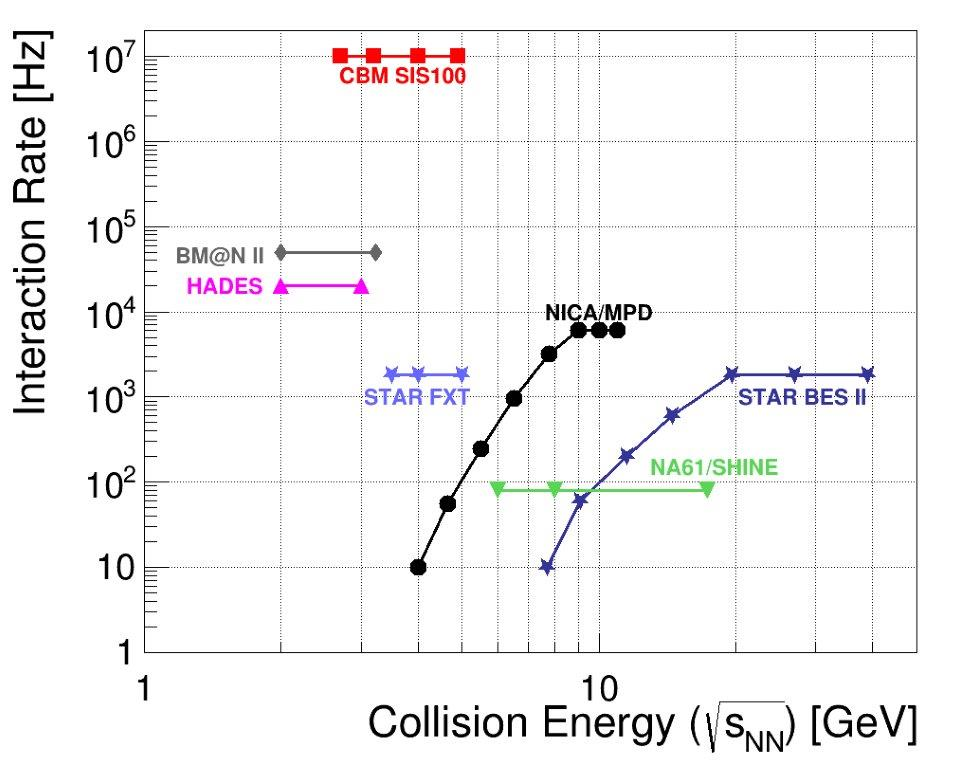
\includegraphics[width=0.8\textwidth]{pictures/Experiments.png}
\caption{Энергии и частоты взаимодействий основных экспериментов, работающих с относительно высокой барионной плотностью. BES --- Beam Energy Scan, FXT --- FiXed Target.}
\label{fig:Experiments}
\end{figure}

Из приведенных данных видно, что эксперимент CBM будет обладать уникальными возможностями по исследованию редких наблюдаемых с высокой статистической точностью. Данная работа посвящена методическим разработкам для детектора RICH эксперимента CBM, участвующего в измерении таких наблюдаемых как распады легких векторных мезонов ($\rho$, $\omega$, $\phi$) и $J/\psi$-частицы по диэлектронному каналу.

\section*{Актуальность работы:}

Современные эксперименты в области физики высоких энергий и, особенно, столкновения релятивистских тяжелых ионов выдвигают жёсткие требования к проектным решениям при создании установок по причине высокой загрузки, высокой плотности потока частиц и высокой радиационной нагрузки, сложности и многопараметричности моделей, описывающих изучаемые эффекты, тонкости последних и высоких фонов.

Например, (рассказать c конкретными цифрами про загрузки, наблюдаемые (измеримые величины) и фоны в ряде экспериментов, в частности, flow measurements и rare probes в CBM, что-то обязательно про СТАР, АЛИСУ и какой-нибудь еще эксперимент с фиксированной мишенью, подчеркнуть особенности и жесткость требований CBM).

Все эти факторы

Требуются совершенные методы моделирования детекторов с высоким уровнем детализации и возможностью выполнения нескольких итераций расчетов, а также разработка новых систем сбора данных, адекватных современному аппаратному обеспечению и ожидаемым потокам информации.

Кроме того, необходимы интенсивные исследования прототипов создаваемых детекторов.

В настоящей диссертации обсуждаются все три перечисленных аспекта (развернуть на 1-2 абзаца) в применении, в первую очередь, к детектору Черенковских колец эксперимента CBM (далее CBM RICH).

\section*{Цели:}

\begin{itemize}
\item{разработать инструментарий для облегчения создания детальных геометрических моделей, предназначенных для таких сред Монте-Карло моделирования прохождения частиц через вещество, как Geant4 и ROOT, а также для обмена геометрической информацией между этими средами и САПР CATIA~v5;}
\item{создать гибкое и точное описание детектора CBM RICH в среде CbmRoot и осуществить на основе этого описания оптимизацию конструкции и компоновки данного детектора;}
\item{создать ПО для испытания прототипа системы считывания и сбора данных детектора CBM RICH в составе полнофункционального прототипа указанного детектора на пучковых тестах;}
\item{провести исследование свойств прототипа системы считывания и сбора данных детектора CBM RICH на основе результатов пучковых тестов и измерений на лабораторном стенде.}
\end{itemize}

\section*{Научная новизна и практическая ценность работы:}

\begin{enumerate}
\item Разработана схема отображения иерархии геометрии, используемой в моделировании транспорта частиц методом Монте-Карло (МК), на дерево построений САПР CATIA~v5.
\item В среде CATIA~v5 создан набор шаблонов для примитивов и сущностей конструктивной твердотельной геометрии, принятой в системах МК моделирования детекторов.
\item Создан набор инструментов для полуавтоматического построения детальной МК геометрии на основе САПР модели и быстрого обмена геометрией между САПР CATIA~v5 и пакетами МК моделирования GEANT и ROOT.
\item Выполнены беспрецедентно точные параметризованные описания ряда приборов и детекторов в средах МК моделирования.
\item На основе детального параметризованного описания геометрии CBM~RICH выполнена оптимизация компоновки детектора. 
\item Собран прототип системы считывания и сбора данных детектора CBM~RICH.
\item Разработано программное обеспечение для приема, упаковки и передачи бестриггерного потока данных с прототипа системы считывания и сбора данных с частотой до 20~МГц.
\item Разработано программное обеспечение для калибровки точного времени и относительных задержек каналов в потоке данных с детектора CBM RICH.
\item Разработано программное обеспечение для построения событий из бестриггерного потока данных с детектора CBM~RICH в среде CbmRoot.
\item Проведены пучковые тесты прототипа системы считывания и сбора данных в составе полнофункционального прототипа детектора CBM~RICH и дополнительные тесты на лабораторном стенде. 
\item Проведено комплексное исследование свойств канала считывания и сбора данных для CBM~RICH, реализованного на основе многоанодного ФЭУ H12700 с системой динодов ``metal channel'', специально разработанных передней электроники типа предусилитель-дискриминатор и высокоточного ВЦП с последующим прямым вводом данных в единую среду моделирования, сбора и анализа данных CbmRoot.
\item Исследованы временные свойства нанесенного на окно МА~ФЭУ сместителя спектра при возбуждении черенковскими фотонами.
\item Изучены возможности работы канала считывания при пониженных порогах.
\item Проведен сравнительный анализ особенностей считывания многоанодного ФЭУ временным и аналоговым трактами.
% \item Исследованы характеристики детектора CBM~RICH с учетом неидеальности геометрии и шумов электроники.
\end{enumerate}

\section*{На защиту выносятся следующие результаты:}

\begin{enumerate}
\item Разработка методологии и реализация ``CATIA-GDML geometry builder'', средства построения сложной, основанной на инженерном дизайне геометрии детекторов для моделирования прохождения и взаимодействия частиц.
\item Применение ``CATIA-GDML geometry builder'' для построения беспрецедентно точного параметризованного описания геометрии CBM~RICH в среде CbmRoot.
\item Реализация прототипа системы считывания и сбора данных CBM~RICH и проведение его тестов на пучке в составе полнофункционального прототипа этого детектора а также дополнительных тестов на лабораторном стенде.
\item Разработка алгоритмов и программного обеспечения для приема, упаковки и передачи бестриггерного потока данных, для калибровки точного времени и относительных задержек каналов и для построения событий из потока данных с детектора CBM RICH в среде CbmRoot.
\item Результаты комплексного исследования временных свойств канала считывания и сбора данных для CBM~RICH, реализованного на основе многоанодного ФЭУ H12700 с системой динодов ``metal channel'', специально разработанных передней электроники типа предусилитель-дискриминатор и высокоточного ВЦП с последующим прямым вводом данных в единую среду моделирования, сбора и анализа данных CbmRoot.
\item Исследование временных свойств нанесенного на окно МА ФЭУ сместителя спектра при возбуждении черенковскими фотонами.
\item Сравнительный анализ особенностей считывания многоанодного ФЭУ временным и аналоговым трактами.
% \item Исследование характеристик детектора CBM~RICH с учетом неидеальности геометрии и шумов электроники.
\end{enumerate}

\section*{Представление основных положений и результатов}

% Приведено в обратном хронологическом порядке. Можно перегруппировать по важности.

Основные положения и результаты работы докладывались и обсуждались на научных семинарах ЛИТ ОИЯИ и на различных международных конференциях и совещаниях, в том числе:

\begin{enumerate}

\item Семинар НОВФ ЛИТ ОИЯИ, Дубна, Россия, 22.12.2016 \\
Устный доклад ``Development of the readout and DAQ system for CBM RICH and EXPERT. 'CATIA-GDML geometry buidler' and Monte-Carlo geometry of CBM RICH.''

\item Семинар ``Contribution of the young Russian scientists into the project FAIR'', ИТЭФ, Москва, Россия, 14-15.12.2016 \\
Устный доклад ``Detailed study of the stability and uniformity of the CBM RICH readout and DAQ prototype characteristics. Development and application of the Monte Carlo geometry package''

\item Международная конференция ``The 9th International Workshop on Ring Imaging Cherenkov Detectors (RICH 2016)'', Блед, Словения, 05-09.09.2016 \\
Представлен постер ``Development of the CBM RICH readout electronics and DAQ''

\item Международная конференция ``The 20th IEEE-NPSS Real Time Conference (IEEE-NPSS RT2016)'', Падуя, Италия, 05-10.06.2016 \\
Представлен постер ``Development of the CBM RICH readout and DAQ''

\item Международная конференция ``The XX International Scientific Conference of Young Scientists and Specialists (AYSS-2016)'', ОИЯИ, Дубна, Россия, 14-18.03.2016 \\
Устный доклад ``Development and characterization of CBM RICH readout and DAQ''

\item Семинар ``Contribution of the young Russian scientists into the project FAIR'', ИТЭФ, Москва, Россия, 15-17.12.2015 \\
Устный доклад ``Development of 'CATIA-GDML geometry builder' and CBM RICH software''

\item Международное совещание ``26th CBM Collaboration Meeting'', Прага, Чехия, 14-18.09.2015 \\
Устный доклад ``PADIWA test measurements, beamtime analysis (TOT, WLS time resolution)''

\item Международное совещание ``25th CBM Collaboration Meeting'', ГСИ, Дармштадт, Германия, 20-24.04.2015 \\
Устный доклад ``Beamtime analysis: FLIB readout, TOT, timing''

\item Семинар ``Contribution of the young Russian scientists into the project FAIR'', ИТЭФ, Москва, Россия, 12-13.11.2013 \\
Устный доклад ``Modernization of simulation and data acquisition packages of CBM experiment''

\item Международная конференция ``20th International Conference on Computing in High Energy and Nuclear Physics (CHEP)'', Амстердам, Нидерланды, 14-18.10.2013 \\
Представлен постер ``Development and application of CATIA-GDML geometry builder''

\end{enumerate}

\section*{Публикации}


\section*{Личный вклад:}

\todo
\section*{Структура и содержание}\label{sec:secStructureAndContent}

Диссертация состоит из настоящего введения, пяти глав и заключения.

В первой главе
описываются условия эксплуатации, компоновка и основные свойства детекторов эксперимента CBM;
обсуждается важность точного описания и оптимизации конструкции детекторов в свете жёстких условий эксплуатации;
формулируется задача разработки инструментария для обмена геометрической информацией между САПР и средами Монте-Карло моделирования прохождения частиц через вещество (Geant4/ROOT) и облегчения создания детальных геометрических моделей для Geant4/ROOT;
детально описывается конструкция детектора CBM RICH и проводится сравнение с аналогичными приборами из ряда других экспериментов;
формулируются конкретные задачи, связанные с описанием геометрии детектора CBM RICH в среде Монте-Карло;
обсуждается концепция системы считывания и сбора данных эксперимента CBM и воплощение этой концепции в системе считывания и сбора данных детектора CBM RICH;
формулируется задача на исследование прототипа системы считывания и сбора данных указанного детектора.

Во второй главе
обсуждаются некоторые наиболее распространённые способы представления геометрических моделей в ЭВМ, используемые в различном ПО для решения различных вычислительных задач;
рассматриваются предпосылки и принципы создания инструментария, так называемого ``CATIA-GDML geometry builder'', для обмена геометрической информацией между САПР и средами Монте Карло моделирования прохождения частиц через вещество (Geant4/ROOT) и облегчения создания детальных геометрических моделей для Geant4/ROOT;
обсуждаются реализация отображения примитивов и иерархии объемов Geant4/ROOT на дерево построений в среде CATIA~v5 и набор созданных макропрограмм, входящих в ``CATIA-GDML geometry builder'';
описывается методика применения ``CATIA-GDML geometry builder'' и приводятся некоторые примеры.

Третья глава
посвящена применению пакета ``CATIA-GDML geometry builder'' для детектора CBM RICH. В ней подробно рассмотрены задачи, требующие точного описания геометрии механических конструкций детектора и системы крепления и позиционирования зеркал, учета эффектов, связанных с отклонением позиционирования зеркал от номинального, размещения и экранирования от магнитного поля фотодетекторов. Описаны созданные параметризованные геометрические модели и проведенные с их помощью исследования свойств детектора CBM RICH. Кроме того, даются рекомендации по эффективному применению использованного инструментария.

В четвёртой главе
описаны архитектура бестриггерной системы считывания и сбора данных CBM RICH, разработанные модули ПО, необходимые для сбора и анализа данных, а также экспериментальные установки, позволившие осуществить всестороннее исследование прототипа указанной системы.

Пятая глава
посвящена анализу данных пучковых и лабораторных тестов прототипа детектора CBM RICH и результатам исследования свойств и характеристик прототипа системы считывания и сбора данных. Здесь же, на основании проведенных исследований, даются рекомендации по модификации следующей версии прототипа системы считывания и сбора данных.

В заключении приводятся основные результаты работы и выражаются благодарности.

